\documentclass[aspectratio=169,10pt]{beamer}

% Compile with: pdflatex slides.tex
% Put generated/reproduced figures in ./figures with the filenames used below.
% Missing figures are rendered as clean placeholders.

\usepackage[utf8]{inputenc}
\usepackage[T1]{fontenc}
\usepackage{helvet}
\usepackage{amsmath,amssymb}
\usepackage{booktabs}
\usepackage{graphicx}
\usepackage{microtype}
\usepackage{tikz}
\usetikzlibrary{arrows.meta,positioning,calc}

\renewcommand{\familydefault}{\sfdefault}
\graphicspath{{figures/}}

% ---------- Modern warm theme ----------
\definecolor{Paper}{HTML}{F8F4EA}
\definecolor{Ink}{HTML}{24211E}
\definecolor{Muted}{HTML}{6D675F}
\definecolor{Coral}{HTML}{D45D4C}
\definecolor{Moss}{HTML}{4C7C59}
\definecolor{Gold}{HTML}{D8A03A}
\definecolor{Panel}{HTML}{FFFFFF}
\definecolor{Line}{HTML}{E2D8C7}
\definecolor{Deep}{HTML}{1F2A24}

\setbeamertemplate{navigation symbols}{}
\setbeamertemplate{itemize item}{\color{Coral}\small$\blacktriangleright$}
\setbeamertemplate{itemize subitem}{\color{Moss}\scriptsize$\bullet$}
\setbeamertemplate{enumerate item}{\color{Coral}\insertenumlabel.}
\setbeamertemplate{caption}[numbered]

\setbeamercolor{normal text}{fg=Ink,bg=Paper}
\setbeamercolor{frametitle}{fg=Ink,bg=Paper}
\setbeamercolor{title}{fg=Ink,bg=Paper}
\setbeamercolor{subtitle}{fg=Muted,bg=Paper}
\setbeamercolor{structure}{fg=Coral}
\setbeamercolor{block title}{fg=Paper,bg=Deep}
\setbeamercolor{block body}{fg=Ink,bg=Panel}
\setbeamercolor{alerted text}{fg=Coral}
\setbeamercolor{footline}{fg=Muted,bg=Paper}

\setbeamerfont{title}{size=\LARGE,series=\bfseries}
\setbeamerfont{subtitle}{size=\normalsize}
\setbeamerfont{frametitle}{size=\Large,series=\bfseries}
\setbeamerfont{framesubtitle}{size=\small}
\setbeamerfont{footline}{size=\scriptsize}

\setbeamertemplate{frametitle}{%
  \vspace{0.25em}
  \begin{tikzpicture}[remember picture,overlay]
    \fill[Gold] ([yshift=-0.08cm]current page.north west)
      rectangle ([xshift=\paperwidth,yshift=-0.11cm]current page.north west);
    \fill[Coral] ([yshift=-0.08cm]current page.north west)
      rectangle ([xshift=0.23\paperwidth,yshift=-0.11cm]current page.north west);
  \end{tikzpicture}
  \insertframetitle\par
  \ifx\insertframesubtitle\empty\else
    {\usebeamerfont{framesubtitle}\color{Muted}\insertframesubtitle\par}
  \fi
  \vspace{-0.35em}
}

\setbeamertemplate{footline}{%
  \leavevmode%
  \hbox{%
    \begin{beamercolorbox}[wd=.72\paperwidth,ht=2.8ex,dp=1.1ex,leftskip=.45cm]{footline}%
      \insertshorttitle
    \end{beamercolorbox}%
    \begin{beamercolorbox}[wd=.28\paperwidth,ht=2.8ex,dp=1.1ex,rightskip=.45cm plus1fil]{footline}%
      \hfill \insertframenumber/\inserttotalframenumber
    \end{beamercolorbox}%
  }%
}

\newcommand{\tagline}[1]{%
  \vspace{0.25em}
  {\color{Muted}\large #1}
}

\newcommand{\keyword}[1]{%
  {\color{Coral}\textbf{#1}}
}

\newcommand{\metric}[2]{%
  \begin{tikzpicture}[baseline=(box.base)]
    \node[fill=Panel,draw=Line,rounded corners=3pt,inner xsep=8pt,inner ysep=6pt] (box)
      {\begin{minipage}{0.82\linewidth}\centering
        {\color{Coral}\Large\bfseries #1}\\[-0.2em]
        {\scriptsize\color{Muted} #2}
      \end{minipage}};
  \end{tikzpicture}
}

\newcommand{\modelcard}[3]{%
  \begin{tikzpicture}
    \node[fill=Panel,draw=Line,rounded corners=4pt,inner sep=10pt,text width=0.92\linewidth] {
      {\large\bfseries #1}\par\vspace{0.35em}
      {\color{Muted} #2}\par\vspace{0.7em}
      #3
    };
  \end{tikzpicture}
}

\newcommand{\figureplaceholder}[2][0.86\linewidth]{%
  \begingroup
  \setlength{\fboxsep}{0pt}%
  \centering
  \fcolorbox{Line}{Panel}{%
    \begin{minipage}[c][0.39\textheight][c]{#1}
      \centering
      {\color{Coral}\Large\bfseries Figure placeholder}\\[0.6em]
      {\small Expected file}\\[0.2em]
      {\ttfamily\scriptsize\detokenize{#2}}\\[0.7em]
      {\scriptsize\color{Muted} Replace by putting the image in the figures directory.}
    \end{minipage}%
  }%
  \endgroup
}

\newcommand{\smartfigure}[3][0.88\linewidth]{%
  \begin{figure}
    \centering
    \IfFileExists{#2}{%
      \includegraphics[width=#1,height=0.45\textheight,keepaspectratio]{#2}%
    }{%
      \figureplaceholder[#1]{#2}%
    }%
    \caption{\scriptsize #3}
  \end{figure}
}

\newcommand{\sectionframe}[2]{%
  {
  \setbeamertemplate{footline}{}
  \begin{frame}[plain]
    \begin{tikzpicture}[remember picture,overlay]
      \fill[Deep] (current page.south west) rectangle (current page.north east);
      \fill[Gold] (current page.south west) rectangle ([xshift=0.24\paperwidth,yshift=0.07\paperheight]current page.south west);
      \fill[Coral] ([xshift=0.24\paperwidth]current page.south west) rectangle ([xshift=0.37\paperwidth,yshift=0.07\paperheight]current page.south west);
    \end{tikzpicture}
    \vfill
    {\color{Gold}\small\bfseries #1}\par\vspace{0.5em}
    {\color{Paper}\Huge\bfseries #2}
    \vfill
  \end{frame}
  }
}

% ---------- Metadata ----------
\title[Superspreaders in Epidemic Spread]{Effects of Superspreaders in Spread of Epidemic}
\subtitle{Introduction to Mathematical Modelling}
\author[Group Banh Thui]{%
  Nguyen Thanh Lam \and Luong Xuan Nguyen \and Nguyen Quan\\
  Nguyen Binh Anh \and Bui Huu Vinh
}
\institute{Hanoi University of Science and Technology}
\date{June 2026}

\begin{document}

% ---------- Title ----------
{
\setbeamertemplate{footline}{}
\begin{frame}[plain]
  \begin{tikzpicture}[remember picture,overlay]
    \fill[Paper] (current page.south west) rectangle (current page.north east);
    \fill[Deep] (current page.south west) rectangle ([xshift=0.39\paperwidth]current page.north west);
    \fill[Coral] ([xshift=0.39\paperwidth]current page.south west) rectangle ([xshift=0.405\paperwidth]current page.north west);
    \fill[Gold] ([xshift=0.405\paperwidth]current page.south west) rectangle ([xshift=0.421\paperwidth]current page.north west);
  \end{tikzpicture}
  \begin{columns}[T,totalwidth=\linewidth]
    \begin{column}{0.32\linewidth}
      \vspace{1.1cm}
      {\color{Paper}\bfseries HUST}\par
      {\color{Gold}\small Introduction to Mathematical Modelling}\par
      \vspace{5.1cm}
      {\color{Paper}\scriptsize Group Banh Thui}\par
      {\color{Paper}\scriptsize Supervisor: Dr. Bui Quoc Trung}
    \end{column}
    \begin{column}{0.60\linewidth}
      \vspace{1.35cm}
      {\usebeamerfont{title}\inserttitle\par}
      \vspace{0.45em}
      {\usebeamerfont{subtitle}\color{Muted} A spatial SIR view of why a few highly connected individuals can reshape an outbreak\par}
      \vspace{1.35cm}
      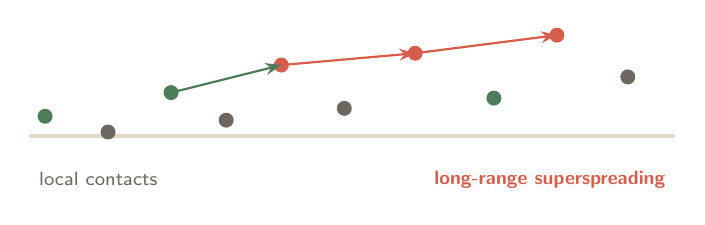
\begin{tikzpicture}[x=1cm,y=1cm]
        \draw[Line,very thick] (0,0) -- (8.2,0);
        \foreach \x/\y/\c in {0.2/0.25/Moss,1.0/0.05/Muted,1.8/0.55/Moss,2.5/0.2/Muted,3.2/0.9/Coral,4.0/0.35/Muted,4.9/1.05/Coral,5.9/0.48/Moss,6.7/1.28/Coral,7.6/0.75/Muted}
          \fill[\c] (\x,\y) circle (2.7pt);
        \draw[Coral,thick,-{Stealth[length=2mm]}] (3.2,0.9) -- (4.9,1.05);
        \draw[Coral,thick,-{Stealth[length=2mm]}] (4.9,1.05) -- (6.7,1.28);
        \draw[Moss,thick,-{Stealth[length=2mm]}] (1.8,0.55) -- (3.2,0.9);
        \node[anchor=west,color=Muted,font=\scriptsize] at (0,-0.55) {local contacts};
        \node[anchor=east,color=Coral,font=\scriptsize\bfseries] at (8.2,-0.55) {long-range superspreading};
      \end{tikzpicture}
      \vfill
      {\color{Muted}\small Fujie and Odagaki, Physica A, 2007 \hfill \insertdate}
    \end{column}
  \end{columns}
\end{frame}
}

\begin{frame}{One-Slide Summary}
  \tagline{Question: how do superspreaders change epidemic spread in a spatial SIR model?}
  \vspace{1.2em}
  \begin{columns}[T,totalwidth=\linewidth]
    \begin{column}{0.48\linewidth}
      \begin{itemize}
        \item Classical SIR assumes similar transmission ability for all infected individuals.
        \item The paper adds \keyword{heterogeneity} through a fraction $\lambda$ of superspreaders.
        \item Two mechanisms are compared: stronger local infectiousness and wider social reach.
      \end{itemize}
    \end{column}
    \begin{column}{0.48\linewidth}
      \begin{block}{Main conclusion}
        Superspreaders lower the density threshold for epidemic percolation, speed up spatial propagation, sharpen epidemic curves, and create long-tailed secondary infection distributions.
      \end{block}
    \end{column}
  \end{columns}
\end{frame}

\begin{frame}{Talk Roadmap}
  \vspace{0.4em}
  \begin{columns}[T,totalwidth=\linewidth]
    \begin{column}{0.24\linewidth}
      \metric{01}{Motivation}
    \end{column}
    \begin{column}{0.24\linewidth}
      \metric{02}{Spatial SIR model}
    \end{column}
    \begin{column}{0.24\linewidth}
      \metric{03}{Monte Carlo solution}
    \end{column}
    \begin{column}{0.24\linewidth}
      \metric{04}{Results and SARS comparison}
    \end{column}
  \end{columns}
  \vspace{1.3em}
  \begin{center}
  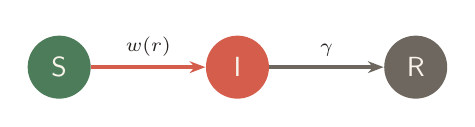
\begin{tikzpicture}[node distance=1.45cm]
    \node[circle,fill=Moss,text=Paper,minimum size=8mm] (s) {S};
    \node[circle,fill=Coral,text=Paper,minimum size=8mm,right=of s] (i) {I};
    \node[circle,fill=Muted,text=Paper,minimum size=8mm,right=of i] (r) {R};
    \draw[very thick,-{Stealth[length=2mm]},Coral] (s) -- node[above,font=\scriptsize,color=Ink] {$w(r)$} (i);
    \draw[very thick,-{Stealth[length=2mm]},Muted] (i) -- node[above,font=\scriptsize,color=Ink] {$\gamma$} (r);
  \end{tikzpicture}
  \end{center}
\end{frame}

\sectionframe{Part 1}{Model}

\begin{frame}{Why Superspreaders Matter}
  \begin{columns}[T,totalwidth=\linewidth]
    \begin{column}{0.52\linewidth}
      \begin{itemize}
        \item In many outbreaks, a small number of infected individuals cause a disproportionate number of secondary infections.
        \item A homogeneous SIR model cannot represent this variance directly.
        \item The paper asks whether epidemic spread is driven more by \keyword{high infectiousness} or by \keyword{high connectivity}.
      \end{itemize}
    \end{column}
    \begin{column}{0.42\linewidth}
      \begin{block}{Reference example}
        The 2003 SARS outbreak contained several superspreading events, including cases in Singapore and Hong Kong.
      \end{block}
      \vspace{0.5em}
      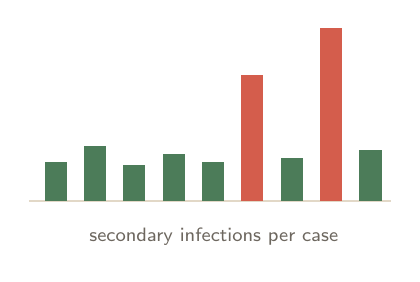
\begin{tikzpicture}
        \draw[Line,thick] (0,0) -- (4.6,0);
        \foreach \x/\h/\c in {0.2/0.5/Moss,0.7/0.7/Moss,1.2/0.45/Moss,1.7/0.6/Moss,2.2/0.5/Moss,2.7/1.6/Coral,3.2/0.55/Moss,3.7/2.2/Coral,4.2/0.65/Moss}
          \fill[\c] (\x,0) rectangle +(0.28,\h);
        \node[color=Muted,font=\scriptsize] at (2.35,-0.45) {secondary infections per case};
      \end{tikzpicture}
    \end{column}
  \end{columns}
\end{frame}

\begin{frame}{Spatial SIR Setting}
  \begin{columns}[T,totalwidth=\linewidth]
    \begin{column}{0.52\linewidth}
      \begin{itemize}
        \item $N$ individuals are fixed in a continuous square domain $L\times L$.
        \item Each individual has state $X_i(t)\in\{S,I,R\}$.
        \item Population density:
        \[
          \rho=\frac{N}{L^2}, \qquad L=10r_0.
        \]
        \item A fraction $\lambda$ of individuals are designated as superspreaders.
      \end{itemize}
    \end{column}
    \begin{column}{0.42\linewidth}
      \centering
      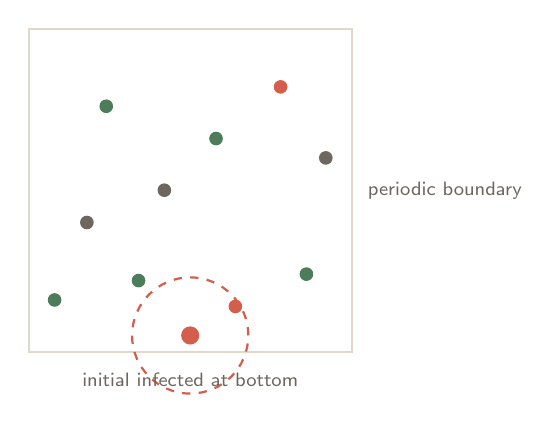
\begin{tikzpicture}[scale=0.82]
        \draw[Line,thick,fill=Panel] (0,0) rectangle (5,5);
        \foreach \x/\y/\c in {0.4/0.8/Moss,1.2/3.8/Moss,2.1/2.5/Muted,3.9/4.1/Coral,4.3/1.2/Moss,0.9/2.0/Muted,2.9/3.3/Moss,3.2/0.7/Coral,1.7/1.1/Moss,4.6/3.0/Muted}
          \fill[\c] (\x,\y) circle (3pt);
        \fill[Coral] (2.5,0.25) circle (4pt);
        \draw[Coral,thick,dashed] (2.5,0.25) circle (0.9);
        \node[below,color=Muted,font=\scriptsize] at (2.5,-0.18) {initial infected at bottom};
        \node[right,color=Muted,font=\scriptsize] at (5.1,2.5) {periodic boundary};
      \end{tikzpicture}
    \end{column}
  \end{columns}
\end{frame}

\begin{frame}{Periodic Distance}
  \tagline{The square behaves like a torus, so boundary effects are reduced.}
  \vspace{0.8em}
  For individuals at $(x_1,y_1)$ and $(x_2,y_2)$:
  \[
    r=
    \sqrt{
      \left(\min(|x_1-x_2|,L-|x_1-x_2|)\right)^2+
      \left(\min(|y_1-y_2|,L-|y_1-y_2|)\right)^2
    }.
  \]
  \vspace{0.8em}
  \begin{block}{Why it matters}
    Infection probability depends on this wrapped distance, not the ordinary Euclidean distance inside a bounded square.
  \end{block}
\end{frame}

\begin{frame}{Transmission and Recovery}
  \begin{columns}[T,totalwidth=\linewidth]
    \begin{column}{0.50\linewidth}
      \begin{itemize}
        \item In each Monte Carlo step, only individuals infected at the start of the step can transmit.
        \item A susceptible individual at distance $r$ is infected with probability $w(r)$.
        \item After attempting transmission, each infected individual recovers with probability $\gamma$.
        \item Reference simulations use $w_0=1$ and $\gamma=1$.
      \end{itemize}
    \end{column}
    \begin{column}{0.44\linewidth}
      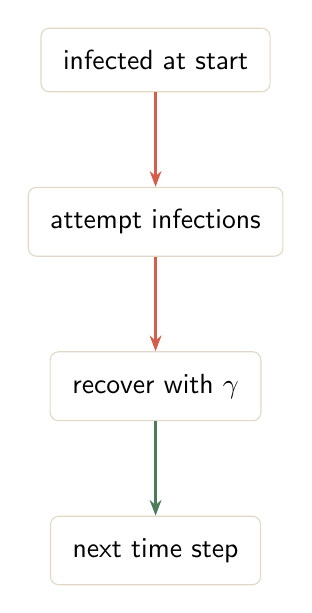
\begin{tikzpicture}[node distance=1.2cm]
        \node[draw=Line,fill=Panel,rounded corners=3pt,inner sep=8pt] (a) {infected at start};
        \node[draw=Line,fill=Panel,rounded corners=3pt,inner sep=8pt,below=of a] (b) {attempt infections};
        \node[draw=Line,fill=Panel,rounded corners=3pt,inner sep=8pt,below=of b] (c) {recover with $\gamma$};
        \node[draw=Line,fill=Panel,rounded corners=3pt,inner sep=8pt,below=of c] (d) {next time step};
        \draw[-{Stealth[length=2mm]},thick,Coral] (a) -- (b);
        \draw[-{Stealth[length=2mm]},thick,Coral] (b) -- (c);
        \draw[-{Stealth[length=2mm]},thick,Moss] (c) -- (d);
      \end{tikzpicture}
    \end{column}
  \end{columns}
\end{frame}

\begin{frame}{Two Superspreader Mechanisms}
  \begin{columns}[T,totalwidth=\linewidth]
    \begin{column}{0.49\linewidth}
      \modelcard{Strong infectiousness}{Same local radius, higher infection probability.}{
        \[
        w_s(r)=
        \begin{cases}
          w_0,&0\le r\le r_0,\\
          0,&r>r_0.
        \end{cases}
        \]
        \begin{center}
          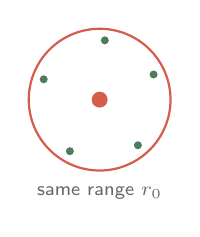
\begin{tikzpicture}[scale=0.72]
            \fill[Coral] (0,0) circle (4pt);
            \draw[Coral,thick] (0,0) circle (1.25);
            \foreach \a in {25,85,160,240,310}
              \fill[Moss] ({1.05*cos(\a)},{1.05*sin(\a)}) circle (2pt);
            \node[color=Muted,font=\scriptsize] at (0,-1.65) {same range $r_0$};
          \end{tikzpicture}
        \end{center}
      }
    \end{column}
    \begin{column}{0.49\linewidth}
      \modelcard{Hub model}{Same probability shape, wider contact range.}{
        \[
        w_s(r)=
        \begin{cases}
          w_0(1-r/r_n)^2,&0\le r\le r_n,\\
          0,&r>r_n,
        \end{cases}
        \]
        \[
          r_n=\sqrt{6}r_0 \quad \text{for superspreaders.}
        \]
      }
    \end{column}
  \end{columns}
\end{frame}

\begin{frame}{Normal vs Superspreader Infection Kernels}
  \begin{columns}[T,totalwidth=\linewidth]
    \begin{column}{0.48\linewidth}
      \begin{block}{Normal infected individual}
        \[
        w_n(r)=
        \begin{cases}
        w_0(1-r/r_0)^2,&0\le r\le r_0,\\
        0,&r>r_0.
        \end{cases}
        \]
      \end{block}
      \vspace{0.6em}
      \begin{itemize}
        \item Local transmission.
        \item Probability decays with distance.
      \end{itemize}
    \end{column}
    \begin{column}{0.48\linewidth}
      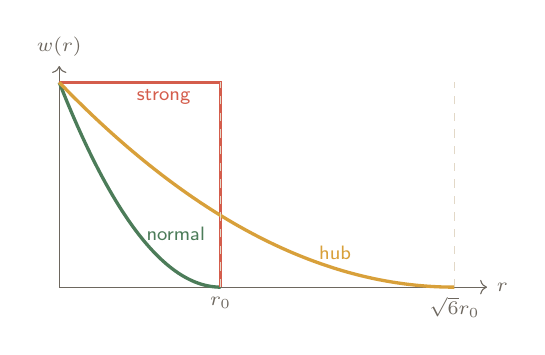
\begin{tikzpicture}[x=2.05cm,y=2.6cm]
        \draw[->,Muted] (0,0) -- (2.65,0) node[right,font=\scriptsize] {$r$};
        \draw[->,Muted] (0,0) -- (0,1.08) node[above,font=\scriptsize] {$w(r)$};
        \draw[very thick,Moss,domain=0:1,samples=80] plot (\x,{(1-\x)^2});
        \draw[very thick,Coral] (0,1) -- (1,1) -- (1,0);
        \draw[very thick,Gold,domain=0:2.449,samples=90] plot ({\x},{(1-\x/2.449)^2});
        \draw[dashed,Line] (1,0) -- (1,1);
        \draw[dashed,Line] (2.449,0) -- (2.449,1);
        \node[below,font=\scriptsize,color=Muted] at (1,0) {$r_0$};
        \node[below,font=\scriptsize,color=Muted] at (2.449,0) {$\sqrt{6}r_0$};
        \node[right,font=\scriptsize,color=Moss] at (0.48,0.26) {normal};
        \node[right,font=\scriptsize,color=Coral] at (0.42,0.93) {strong};
        \node[right,font=\scriptsize,color=Gold] at (1.55,0.17) {hub};
      \end{tikzpicture}
      \vspace{0.6em}
      \begin{block}{Normalization idea}
        The hub radius $\sqrt{6}r_0$ makes the expected infection strength comparable to the strong infectiousness model.
      \end{block}
    \end{column}
  \end{columns}
\end{frame}

\begin{frame}{Basic Reproductive Number}
  \tagline{$R_0(\lambda)$ links microscopic infection kernels to the density threshold.}
  \vspace{0.4em}
  \[
  R_0(\lambda)
  =
  \frac{\rho}{w_0}
  \left[
    \lambda \int w_s(r)2\pi r\,dr+
    (1-\lambda)\int w_n(r)2\pi r\,dr
  \right].
  \]
  \vspace{0.4em}
  Percolation threshold:
  \[
    R_0=R_c,
    \qquad
    \rho_c\pi r_0^2
    =
    \frac{R_c}{\lambda+\frac{1-\lambda}{6}}.
  \]
  \vspace{0.6em}
  \begin{columns}[T,totalwidth=\linewidth]
    \begin{column}{0.48\linewidth}
      \begin{block}{Strong infectiousness}
        $R_c \approx 4.5$
      \end{block}
    \end{column}
    \begin{column}{0.48\linewidth}
      \begin{block}{Hub model}
        $R_c \approx 3.2$
      \end{block}
    \end{column}
  \end{columns}
\end{frame}

\sectionframe{Part 2}{Solving Algorithm}

\begin{frame}{Monte Carlo Simulation}
  \begin{columns}[T,totalwidth=\linewidth]
    \begin{column}{0.50\linewidth}
      \begin{enumerate}
        \item Initialize positions, states, and superspreader labels.
        \item For each infected individual, test infection against all susceptible individuals.
        \item Record new infections, infection parent, front distance, and secondary infection count.
        \item Recover current infected individuals with probability $\gamma$.
        \item Stop when no infected individuals remain.
      \end{enumerate}
    \end{column}
    \begin{column}{0.44\linewidth}
      \begin{block}{Output quantities}
        \begin{itemize}
          \item percolation probability
          \item propagation front $r_f(t)$
          \item epidemic curve
          \item secondary infection distribution
        \end{itemize}
      \end{block}
    \end{column}
  \end{columns}
\end{frame}

\begin{frame}{Simulation Parameters}
  \centering
  \begin{tabular}{lll}
    \toprule
    Quantity & Meaning & Reference setting \\
    \midrule
    $N$ & number of individuals & 150 to 900 \\
    $L$ & domain side length & $10r_0$ \\
    $w_0$ & max infection probability & 1 \\
    $\gamma$ & recovery probability & 1 \\
    $\lambda$ & superspreader fraction & varied \\
    $\rho\pi r_0^2$ & dimensionless density & varied \\
    \bottomrule
  \end{tabular}
  \vspace{1em}
  \begin{block}{Interpretation}
    Increasing $\lambda$ changes the structure of the infection network even when the average infection strength is normalized.
  \end{block}
\end{frame}

\sectionframe{Part 3}{Results}

\begin{frame}{Result 1: Percolation Probability}
  \smartfigure{figures/fig1_strong_percolation.png}{Percolation probability versus density for different superspreader fractions in the strong infectiousness model.}
  \vspace{-0.4em}
  \begin{itemize}
    \item Higher $\lambda$ shifts the transition to lower density.
    \item Epidemic spread becomes possible even in sparser populations.
  \end{itemize}
\end{frame}

\begin{frame}{Result 2: Critical Density}
  \smartfigure{figures/fig3_critical_density.png}{Critical density $\rho_c\pi r_0^2$ as a function of superspreader fraction $\lambda$.}
  \vspace{-0.4em}
  \begin{block}{Reading the curve}
    The hub model has a lower critical density because long-range contacts form transmission paths more easily than purely local strong infectiousness.
  \end{block}
\end{frame}

\begin{frame}{Result 3: Propagation Speed}
  \begin{columns}[T,totalwidth=\linewidth]
    \begin{column}{0.50\linewidth}
      \smartfigure[0.95\linewidth]{figures/fig4_propagation_front_strong.png}{Propagation front distance $r_f/r_0$ over time.}
    \end{column}
    \begin{column}{0.46\linewidth}
      \begin{itemize}
        \item $r_f(t)$ measures the furthest infected individual from the initial case.
        \item The velocity is estimated from the early linear part before finite-size saturation.
        \item The hub model produces faster spread for any $\lambda>0$.
      \end{itemize}
      \vspace{0.4em}
      \smartfigure[0.95\linewidth]{figures/fig5_velocity.png}{Propagation velocity versus $\lambda$.}
    \end{column}
  \end{columns}
\end{frame}

\begin{frame}{Result 4: Epidemic Curves}
  \smartfigure{figures/fig6_epidemic_curves.png}{New infections per time step for no superspreaders, strong infectiousness, and hub model.}
  \vspace{-0.4em}
  \begin{itemize}
    \item Without superspreaders: broader curve, later peak.
    \item With superspreaders: faster growth and sharper peak.
    \item Hub model: earliest and most concentrated outbreak.
  \end{itemize}
\end{frame}

\begin{frame}{Result 5: Secondary Infections}
  \begin{columns}[T,totalwidth=\linewidth]
    \begin{column}{0.48\linewidth}
      \smartfigure[0.96\linewidth]{figures/fig7_link_distribution_no_superspreaders.png}{Distribution without superspreaders.}
    \end{column}
    \begin{column}{0.48\linewidth}
      \smartfigure[0.96\linewidth]{figures/fig8_link_distribution_superspreaders.png}{Distribution with superspreaders.}
    \end{column}
  \end{columns}
  \vspace{-0.4em}
  \begin{block}{Signature of superspreading}
    Many infected individuals cause zero or few secondary cases, while a small number cause many.
  \end{block}
\end{frame}

\begin{frame}{SARS Comparison}
  \begin{columns}[T,totalwidth=\linewidth]
    \begin{column}{0.49\linewidth}
      \smartfigure[0.96\linewidth]{figures/fig9_sars_secondary_cases.png}{Direct secondary cases in the 2003 SARS outbreak in Singapore.}
    \end{column}
    \begin{column}{0.49\linewidth}
      \smartfigure[0.96\linewidth]{figures/fig10_sars_epidemic_comparison.png}{SARS epidemic curve compared with model simulations.}
    \end{column}
  \end{columns}
  \vspace{-0.3em}
  \begin{itemize}
    \item The SARS secondary case distribution is long-tailed.
    \item The hub model gives the best qualitative match to the Singapore epidemic curve.
  \end{itemize}
\end{frame}

\sectionframe{Part 4}{Discussion}

\begin{frame}{What the Model Teaches}
  \begin{columns}[T,totalwidth=\linewidth]
    \begin{column}{0.50\linewidth}
      \begin{block}{Sensitivity}
        Results are sensitive to $\lambda$, population density, and the assumed superspreading mechanism.
      \end{block}
      \begin{itemize}
        \item More superspreaders lower the percolation threshold.
        \item More superspreaders increase propagation speed.
        \item Connectivity changes spatial patterns, not only average case counts.
      \end{itemize}
    \end{column}
    \begin{column}{0.44\linewidth}
      \begin{block}{Limitations}
        \begin{itemize}
          \item individuals are fixed in space
          \item infection probability is simplified
          \item superspreader labels are random
          \item real behavior and interventions are not modeled
        \end{itemize}
      \end{block}
    \end{column}
  \end{columns}
\end{frame}

\begin{frame}{Conclusion}
  \begin{columns}[T,totalwidth=\linewidth]
    \begin{column}{0.52\linewidth}
      \begin{itemize}
        \item Superspreaders strongly reshape epidemic dynamics.
        \item The hub model spreads faster than the strong infectiousness model.
        \item SARS data qualitatively supports long-tailed transmission and high-connectivity explanations.
      \end{itemize}
    \end{column}
    \begin{column}{0.42\linewidth}
      \begin{block}{Key message}
        In this paper, superspreading is not just "more infectiousness"; it is more convincingly modeled as \keyword{greater connectivity}.
      \end{block}
      \vspace{0.8em}
      \centering
      {\Large\bfseries Thank you}
    \end{column}
  \end{columns}
\end{frame}

\begin{frame}{References}
  \small
  \begin{thebibliography}{9}
    \bibitem{fujie2007}
    R. Fujie and T. Odagaki.
    \newblock Effects of superspreaders in spread of epidemic.
    \newblock \emph{Physica A: Statistical Mechanics and its Applications}, 374(2):843--852, 2007.

    \bibitem{lipsitch2003}
    M. Lipsitch et al.
    \newblock Transmission dynamics and control of severe acute respiratory syndrome.
    \newblock \emph{Science}, 300(5627):1966--1970, 2003.
  \end{thebibliography}
\end{frame}

\end{document}
